% Created by tikzDevice version 0.10.1 on 2016-09-02 12:42:34
% !TEX encoding = UTF-8 Unicode
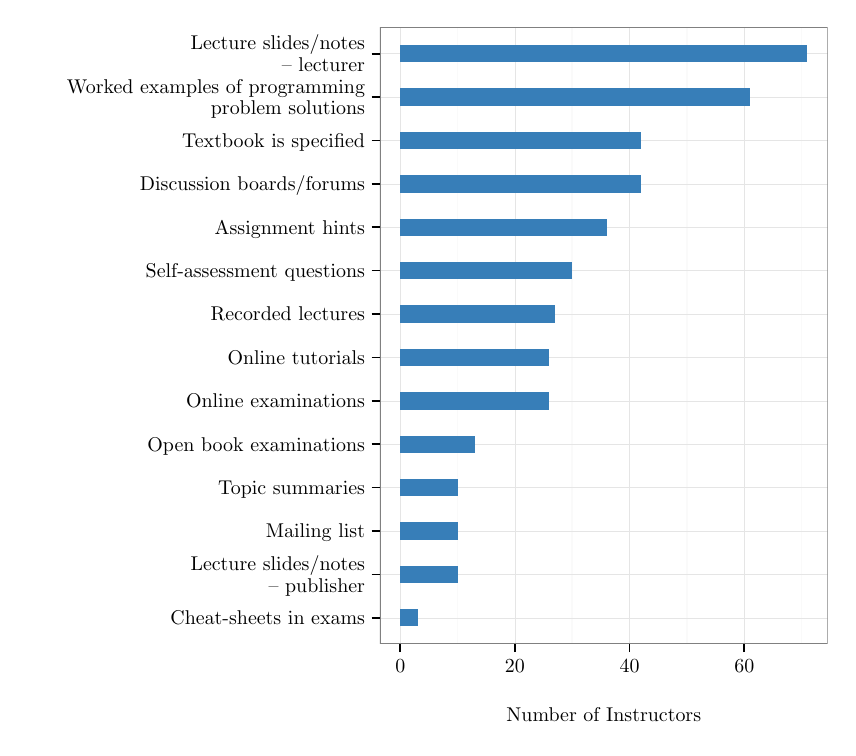
\begin{tikzpicture}[x=1pt,y=1pt]
\definecolor{fillColor}{RGB}{255,255,255}
\path[use as bounding box,fill=fillColor,fill opacity=0.00] (0,0) rectangle (289.08,252.94);
\begin{scope}
\path[clip] (  0.00,  0.00) rectangle (289.08,252.94);
\definecolor{drawColor}{RGB}{255,255,255}
\definecolor{fillColor}{RGB}{255,255,255}

\path[draw=drawColor,line width= 0.6pt,line join=round,line cap=round,fill=fillColor] (  0.00,  0.00) rectangle (289.08,252.95);
\end{scope}
\begin{scope}
\path[clip] (127.30, 30.29) rectangle (289.08,252.94);
\definecolor{fillColor}{RGB}{255,255,255}

\path[fill=fillColor] (127.30, 30.29) rectangle (289.08,252.94);
\definecolor{drawColor}{gray}{0.98}

\path[draw=drawColor,line width= 0.6pt,line join=round] (155.37, 30.29) --
	(155.37,252.94);

\path[draw=drawColor,line width= 0.6pt,line join=round] (196.80, 30.29) --
	(196.80,252.94);

\path[draw=drawColor,line width= 0.6pt,line join=round] (238.23, 30.29) --
	(238.23,252.94);

\path[draw=drawColor,line width= 0.6pt,line join=round] (279.65, 30.29) --
	(279.65,252.94);
\definecolor{drawColor}{gray}{0.90}

\path[draw=drawColor,line width= 0.2pt,line join=round] (127.30, 39.70) --
	(289.08, 39.70);

\path[draw=drawColor,line width= 0.2pt,line join=round] (127.30, 55.38) --
	(289.08, 55.38);

\path[draw=drawColor,line width= 0.2pt,line join=round] (127.30, 71.06) --
	(289.08, 71.06);

\path[draw=drawColor,line width= 0.2pt,line join=round] (127.30, 86.74) --
	(289.08, 86.74);

\path[draw=drawColor,line width= 0.2pt,line join=round] (127.30,102.42) --
	(289.08,102.42);

\path[draw=drawColor,line width= 0.2pt,line join=round] (127.30,118.10) --
	(289.08,118.10);

\path[draw=drawColor,line width= 0.2pt,line join=round] (127.30,133.78) --
	(289.08,133.78);

\path[draw=drawColor,line width= 0.2pt,line join=round] (127.30,149.46) --
	(289.08,149.46);

\path[draw=drawColor,line width= 0.2pt,line join=round] (127.30,165.14) --
	(289.08,165.14);

\path[draw=drawColor,line width= 0.2pt,line join=round] (127.30,180.82) --
	(289.08,180.82);

\path[draw=drawColor,line width= 0.2pt,line join=round] (127.30,196.50) --
	(289.08,196.50);

\path[draw=drawColor,line width= 0.2pt,line join=round] (127.30,212.18) --
	(289.08,212.18);

\path[draw=drawColor,line width= 0.2pt,line join=round] (127.30,227.86) --
	(289.08,227.86);

\path[draw=drawColor,line width= 0.2pt,line join=round] (127.30,243.54) --
	(289.08,243.54);

\path[draw=drawColor,line width= 0.2pt,line join=round] (134.65, 30.29) --
	(134.65,252.94);

\path[draw=drawColor,line width= 0.2pt,line join=round] (176.08, 30.29) --
	(176.08,252.94);

\path[draw=drawColor,line width= 0.2pt,line join=round] (217.51, 30.29) --
	(217.51,252.94);

\path[draw=drawColor,line width= 0.2pt,line join=round] (258.94, 30.29) --
	(258.94,252.94);
\definecolor{fillColor}{RGB}{55,126,184}

\path[fill=fillColor] (134.65, 36.57) rectangle (140.87, 42.84);

\path[fill=fillColor] (134.65, 52.25) rectangle (155.37, 58.52);

\path[fill=fillColor] (134.65, 67.92) rectangle (155.37, 74.20);

\path[fill=fillColor] (134.65, 83.60) rectangle (155.37, 89.88);

\path[fill=fillColor] (134.65, 99.28) rectangle (161.58,105.56);

\path[fill=fillColor] (134.65,114.96) rectangle (188.51,121.24);

\path[fill=fillColor] (134.65,130.64) rectangle (188.51,136.92);

\path[fill=fillColor] (134.65,146.32) rectangle (190.58,152.60);

\path[fill=fillColor] (134.65,162.00) rectangle (196.80,168.27);

\path[fill=fillColor] (134.65,177.68) rectangle (209.23,183.95);

\path[fill=fillColor] (134.65,193.36) rectangle (221.65,199.63);

\path[fill=fillColor] (134.65,209.04) rectangle (221.65,215.31);

\path[fill=fillColor] (134.65,224.72) rectangle (261.01,230.99);

\path[fill=fillColor] (134.65,240.40) rectangle (281.73,246.67);
\definecolor{drawColor}{gray}{0.50}

\path[draw=drawColor,line width= 0.6pt,line join=round,line cap=round] (127.30, 30.29) rectangle (289.08,252.94);
\end{scope}
\begin{scope}
\path[clip] (  0.00,  0.00) rectangle (289.08,252.94);
\definecolor{drawColor}{RGB}{0,0,0}

\node[text=drawColor,anchor=base east,inner sep=0pt, outer sep=0pt, scale=  0.72] at (121.90, 37.22) {Cheat-sheets in exams};

\node[text=drawColor,anchor=base east,inner sep=0pt, outer sep=0pt, scale=  0.72] at (121.90, 56.79) {Lecture slides/notes};

\node[text=drawColor,anchor=base east,inner sep=0pt, outer sep=0pt, scale=  0.72] at (121.90, 49.01) {-- publisher};

\node[text=drawColor,anchor=base east,inner sep=0pt, outer sep=0pt, scale=  0.72] at (121.90, 68.58) {Mailing list};

\node[text=drawColor,anchor=base east,inner sep=0pt, outer sep=0pt, scale=  0.72] at (121.90, 84.26) {Topic summaries};

\node[text=drawColor,anchor=base east,inner sep=0pt, outer sep=0pt, scale=  0.72] at (121.90, 99.94) {Open book examinations};

\node[text=drawColor,anchor=base east,inner sep=0pt, outer sep=0pt, scale=  0.72] at (121.90,115.62) {Online examinations};

\node[text=drawColor,anchor=base east,inner sep=0pt, outer sep=0pt, scale=  0.72] at (121.90,131.30) {Online tutorials};

\node[text=drawColor,anchor=base east,inner sep=0pt, outer sep=0pt, scale=  0.72] at (121.90,146.98) {Recorded lectures};

\node[text=drawColor,anchor=base east,inner sep=0pt, outer sep=0pt, scale=  0.72] at (121.90,162.66) {Self-assessment questions};

\node[text=drawColor,anchor=base east,inner sep=0pt, outer sep=0pt, scale=  0.72] at (121.90,178.34) {Assignment hints};

\node[text=drawColor,anchor=base east,inner sep=0pt, outer sep=0pt, scale=  0.72] at (121.90,194.02) {Discussion boards/forums};

\node[text=drawColor,anchor=base east,inner sep=0pt, outer sep=0pt, scale=  0.72] at (121.90,209.70) {Textbook is specified};

\node[text=drawColor,anchor=base east,inner sep=0pt, outer sep=0pt, scale=  0.72] at (121.90,229.27) {Worked examples of programming};

\node[text=drawColor,anchor=base east,inner sep=0pt, outer sep=0pt, scale=  0.72] at (121.90,221.49) {problem solutions};

\node[text=drawColor,anchor=base east,inner sep=0pt, outer sep=0pt, scale=  0.72] at (121.90,244.95) {Lecture slides/notes};

\node[text=drawColor,anchor=base east,inner sep=0pt, outer sep=0pt, scale=  0.72] at (121.90,237.17) {-- lecturer};
\end{scope}
\begin{scope}
\path[clip] (  0.00,  0.00) rectangle (289.08,252.94);
\definecolor{drawColor}{RGB}{0,0,0}

\path[draw=drawColor,line width= 0.6pt,line join=round] (124.30, 39.70) --
	(127.30, 39.70);

\path[draw=drawColor,line width= 0.6pt,line join=round] (124.30, 55.38) --
	(127.30, 55.38);

\path[draw=drawColor,line width= 0.6pt,line join=round] (124.30, 71.06) --
	(127.30, 71.06);

\path[draw=drawColor,line width= 0.6pt,line join=round] (124.30, 86.74) --
	(127.30, 86.74);

\path[draw=drawColor,line width= 0.6pt,line join=round] (124.30,102.42) --
	(127.30,102.42);

\path[draw=drawColor,line width= 0.6pt,line join=round] (124.30,118.10) --
	(127.30,118.10);

\path[draw=drawColor,line width= 0.6pt,line join=round] (124.30,133.78) --
	(127.30,133.78);

\path[draw=drawColor,line width= 0.6pt,line join=round] (124.30,149.46) --
	(127.30,149.46);

\path[draw=drawColor,line width= 0.6pt,line join=round] (124.30,165.14) --
	(127.30,165.14);

\path[draw=drawColor,line width= 0.6pt,line join=round] (124.30,180.82) --
	(127.30,180.82);

\path[draw=drawColor,line width= 0.6pt,line join=round] (124.30,196.50) --
	(127.30,196.50);

\path[draw=drawColor,line width= 0.6pt,line join=round] (124.30,212.18) --
	(127.30,212.18);

\path[draw=drawColor,line width= 0.6pt,line join=round] (124.30,227.86) --
	(127.30,227.86);

\path[draw=drawColor,line width= 0.6pt,line join=round] (124.30,243.54) --
	(127.30,243.54);
\end{scope}
\begin{scope}
\path[clip] (  0.00,  0.00) rectangle (289.08,252.94);
\definecolor{drawColor}{RGB}{0,0,0}

\path[draw=drawColor,line width= 0.6pt,line join=round] (134.65, 27.29) --
	(134.65, 30.29);

\path[draw=drawColor,line width= 0.6pt,line join=round] (176.08, 27.29) --
	(176.08, 30.29);

\path[draw=drawColor,line width= 0.6pt,line join=round] (217.51, 27.29) --
	(217.51, 30.29);

\path[draw=drawColor,line width= 0.6pt,line join=round] (258.94, 27.29) --
	(258.94, 30.29);
\end{scope}
\begin{scope}
\path[clip] (  0.00,  0.00) rectangle (289.08,252.94);
\definecolor{drawColor}{RGB}{0,0,0}

\node[text=drawColor,anchor=base,inner sep=0pt, outer sep=0pt, scale=  0.72] at (134.65, 19.93) {0};

\node[text=drawColor,anchor=base,inner sep=0pt, outer sep=0pt, scale=  0.72] at (176.08, 19.93) {20};

\node[text=drawColor,anchor=base,inner sep=0pt, outer sep=0pt, scale=  0.72] at (217.51, 19.93) {40};

\node[text=drawColor,anchor=base,inner sep=0pt, outer sep=0pt, scale=  0.72] at (258.94, 19.93) {60};
\end{scope}
\begin{scope}
\path[clip] (  0.00,  0.00) rectangle (289.08,252.94);
\definecolor{drawColor}{RGB}{0,0,0}

\node[text=drawColor,anchor=base,inner sep=0pt, outer sep=0pt, scale=  0.72] at (208.19, 10.18) {};

\node[text=drawColor,anchor=base,inner sep=0pt, outer sep=0pt, scale=  0.72] at (208.19,  2.40) {Number of Instructors};
\end{scope}
\end{tikzpicture}
